\documentclass[14pt]{extarticle}
\usepackage[english]{babel}
\usepackage[utf8x]{inputenc}
\usepackage[T1]{fontenc}
\usepackage{scribe}
\usepackage{listings}
\usepackage{relsize}
\usepackage{xlop}
\usepackage{multirow,bigdelim,dcolumn,booktabs}
\usepackage[linesnumbered,vlined]{algorithm2e}
\usepackage{tikz}
\usepackage{float}
\usetikzlibrary{trees}
\usetikzlibrary{positioning}
\usetikzlibrary{arrows,shapes,automata,petri,positioning,calc,arrows.meta}
\tikzset{
    >=Stealth, % makes the arrow heads bold
    every state/.style={thick},
    every  edge/.append style={->, thick, font=\footnotesize},
}

\Scribe{Aditya Diwakar}
\Lecturer{Frederic Faulkner}
\LectureNumber{7}
\LectureDate{February 1, 2022}
\LectureTitle{Dynamic Programming}

\newcommand{\Mod}[1]{\ (\mathrm{mod}\ #1)}
\newcommand\mycommfont[1]{\footnotesize\ttfamily\textcolor{blue}{#1}}
\SetCommentSty{mycommfont}

\lstset{style=mystyle}
\setlength{\parindent}{0pt}

\begin{document}
	\MakeScribeTop
    
    The exam was moved to Feb 10. You can bring a single sheet of normal
    printer paper (single side, handwritten). Topics cover Lectures 1-6.

    \section*{Dynamic Programming}
    Using a normal approach, how long does it take to compute the Fibonacci
    sequence? The sequence goes like $1, 1, 2, 3, 5, 8, 13, \ldots$ where
    the $nth$ term is the sum of the $(n-1)$ and $(n-2)th$ term.\\

    A naive algorithm for this could be given by the following algorithm:

    \begin{algorithm}[H]
        \SetKwFunction{FMain}{Fib}
        \SetKwProg{Fn}{Function}{:}{}
        \Fn{\FMain{$n$}}{
            \If{$n = 0\lor n = 1$}{
                \Return $1$
            }
            \Return $\Call{\FMain{$n-1$}} + \Call{\FMain{$n-2$}}$
        }
    \end{algorithm}

    For example, let us compute the recursive tree for $Fib(7)$:
    \begin{center}
        \begin{tikzpicture}[level distance=1cm,
          level 1/.style={sibling distance=7cm},
          level 2/.style={sibling distance=4cm},
          level 3/.style={sibling distance=2cm},
          level 4/.style={sibling distance=1cm},
          level 5/.style={sibling distance=.5cm}]
          \node {$7$}
            child {node {$6$}
              child {node {$5$}
                  child {node {$4$}
                      child {node {$3$}
                          child {node {$2$}}
                          child {node {$1$}}
                      }
                      child {node {$2$}}
                  }
                  child {node {$3$}
                      child {node {$2$}}
                      child {node {$1$}}
                  }
              }
              child {node {$4$}
                  child {node {$3$}
                      child {node {$2$}}
                      child {node {$1$}}
                  }
                  child {node {$2$}}
              }
            }
            child {node {$5$}
              child {node {$4$}
                  child {node {$3$}
                      child {node {$2$}}
                      child {node {$1$}}
                  }
                  child {node {$2$}}
              }
              child {node {$3$}
                  child {node {$2$}}
                  child {node {$1$}}
              }
            };
        \end{tikzpicture}
    \end{center}

    This tree contains an exponential amount of work, but also a lot of
    wasted work as we are recomputing many duplicate values (that were
    already computed before).\\

    For example, we are completely recomputing the entire recursive
    tree for $Fib(5)$ on the left most node on level $3$ when it is already
    being computed as the right most node on level $2$.\\

    A better approach is to use \textit{dynamic programming} where we start
    with an empty list and build up the answer from there (being able to 
    remember the computation for smaller subproblems).\\

    In the following algorithm, we initialize a list and include the two
    base cases in the first two enties (first index is $1$). There are no
    recursive calls, but we are still exploiting the recursive structure
    of the problem.

    \begin{algorithm}[H]
        \SetKwFunction{FMain}{Fib}
        \SetKwProg{Fn}{Function}{:}{}
        \Fn{\FMain{$n$}}{
            $T \gets []$\\
            $T[1] \gets 1$\\
            $T[2] \gets 1$\\
            \For{$i\in 2\to n$}{
                $T[i] \gets T[i-1] + T[i-2]$
            }
            \Return $T[n]$
        }
    \end{algorithm}

    \vspace{3mm}
    In general, dynamic programming is great because
    \begin{itemize}
        \item Exploiting recursive structure without recursion
        \item Solve the smaller problems first and store the solutions
            to avoid recalculation
    \end{itemize}
    \vspace{6mm}

    Let's see another example on the next page!

    \pagebreak

    \subsection*{Route Planning Example}
    Let's say you have a start and end point in a grid, and you are curious
    about how long it takes to get from the start to the end.\\

    \begin{center}
        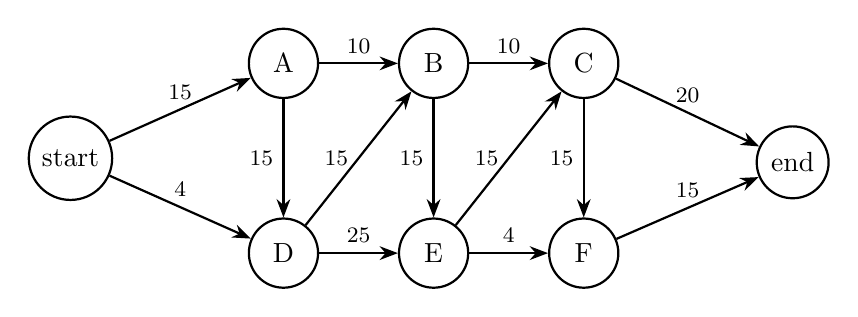
\begin{tikzpicture}
            \node[state] (s) {start};

            % top branch
            \node[state, above right=0.5cm and 2cm of s] (d1) {A};
            \node[state, right=1cm of d1] (d2) {B};
            \node[state, right=1cm of d2] (d3) {C};

            % bottom branch
            \node[state, below right=0.5cm and 2cm of s] (s1) {D};
            \node[state, right=1cm of s1] (s2) {E};
            \node[state, right=1cm of s2] (s3) {F};

            \node[state, above right=0.5cm and 2cm of s3] (u) {end};

            \draw
            (s) edge[above] node{15} (d1)
            (d1) edge[above] node{10} (d2)
            (d2) edge[above] node{10} (d3)
            (d3) edge[above] node{20} (u)

            (s) edge[above] node{4} (s1)
            (s1) edge[above] node{25} (s2)
            (s2) edge[above] node{4} (s3)
            (s3) edge[above] node{15} (u)

            (d1) edge[left] node{15} (s1)
            (s1) edge[left] node{15} (d2)
            (d2) edge[left] node{15} (s2)
            (s2) edge[left] node{15} (d3)
            (d3) edge[left] node{15} (s3)

            ;
        \end{tikzpicture}
    \end{center}

    If we pick the two nodes (colored red and blue), then the time that
    it takes to get to the end can be defined recurively ($T$ is the time it
    takes to get to a certain node):
    \begin{align*}
        T(\texttt{end})  = \min(T(A) + 20, T(B) + 15)
    \end{align*}
    
    A recursive approach this would have a lot of wasted computation 
    (recomputing the distance to nodes we already have a stored value for).
    Rather, we opt for a dynamic programming approach.\\

    \textbf{Idea:} Since we need all the subproblems, calculate the subproblems
    first and then use those to propogate up the problem (larger and larger
    problems).\\

    First, we know that $T(\texttt{start}) = 0$, then $T(A) = 15$ and
    $T(D) = min(T(A) + 15, 4) = 4$. Repeating this logic gives us:
    \begin{align*}
        T(\texttt{start})   &= 0                                \\
        T(A)                &= T(\texttt{start}) + 15 = 15      \\
        T(D)                &= \min(T(\texttt{start}) + 4, T(A) + 15) = 
                                \min(4, 19) = 4                 \\
        T(B)                &= \min(T(A) + 10, T(D) + 15) = \min(25, 19) = 19\\
        T(E)                &= \min(T(B) + 15, T(D) + 25) = \min(34, 29) = 29\\
        T(C)                &= \min(T(B) + 10, T(E) + 15) = \min(29, 44) = 29\\
        T(F)                &= \min(T(E) + 4, T(C) + 15) = \min(33, 44) = 33\\
        T(\texttt{end})     &= \min(T(C) + 20, T(F) + 15) = \min(49, 48) = 
                                \boxed{48}
    \end{align*}

    To formalize this example into an algorithm: the shortest path in a DAG
    (Directed Acyclic Graph) is:

    \begin{algorithm}[H]
        \SetKwFunction{FMain}{ShortestPath}
        \SetKwFunction{Topo}{TopoSort}
        \SetKwProg{Fn}{Function}{:}{}
        \Fn{\FMain{$G, u$}}{
            \tcc{topologically sort the DAG, covered in Unit 3 of this course}
            $G_T \gets \Call{\Topo($G$)}$
            \tcp*{graph is now "ordered"}
            $T\gets \{\}$ \tcp*{dynamic programming map <edge: time>}
            $T[s]\gets 0$ \tcp*{takes no time to get to start}
            \For{$\mathrm{edge}(x, v) \in G$}{
                \tcc{checking if there is a faster way get to $v$}
                $T[v] \gets \min(T[v], T[x] + \mathrm{weight}(x, v))$
            }
            \Return $T[v]$
        }
    \end{algorithm}
    
    The running time for the \texttt{TopoSort} is $O(n^2)$ where $n$ is
    the number of vertices, and there can be as many as $|V|^2 = n^2$ edges,
    so the loop iterates a total of $n^2$ times gives $O(n^2)$ total runtime.

    \subsection*{Dynamically Robbing Houses Example}
    You have houses $h_1, \ldots, h_n$ where $h_i$ is the amount of the
    $i^{th}$ house. You are a robber and cannot rob consecutive houses.
    What is the maximum wealth you can accure?\\

    For every dynamic programming problem, there are 4 parts for a total 
    answer:
    \begin{enumerate}
        \item Table entry definition
        \item Recursive relationship between entries of the table
        \item Pseudocode (for the algorithm, this unit only)
        \item Running time analysis
    \end{enumerate}

    Let $T[i]$ be the maximum wealth from houses $m_1, \ldots, m_i$ (this
    is the table entry definition). Now, we want to know how to define
    $T[i]$ in terms of smaller $i$.\\

    We could choose to rob the $i^{th}$ house, but then we could not
    rob the previous house, so our sum would be $T[i] = h_i + T[i-2]$. However,
    we could also choose not to rob this house, so $T[i] = T[i-1]$ and since
    we want to maximize how much money to make, the recursive relationship
    between entries would be defined as:
    \begin{align*}
        T[i] = \max(h_1 + T[i-2], T[i-1])
    \end{align*}

    For pseudocode, we can implement this as:

    \begin{algorithm}[H]
        \SetKwFunction{FMain}{Robbery}
        \SetKwProg{Fn}{Function}{:}{}
        \Fn{\FMain{$h_1, \ldots, h_n$}}{
            \tcc{let $T$ be an empty array that is $n$ in length}
            $T\gets []$ \\
            $T[1] \gets h_1$
            $T[2] \gets \max(h_1, h_2)$ \\
            \tcc{this loop is inclusive on $n$}
            \For{$i\in 3\to n$}{
                $T[i] \gets \max(h_1 + T[i-2], T[i-1])$
            }
            \Return $T[n]$
        }
    \end{algorithm}

    This algorithm has a total runtime given by $O(n)$ because all operations
    are $O(1)$ while the loop is iterating $O(n)$ times meaning we are making
    $O(n)\ O(1)$ operations, giving $O(n)$ final runtime.

    \subsection*{Challenge: Hopscotch Example}
    Let's play a game of hopscotch! There is a straight line of squares with
    integers values on each square. We start at the start and eventually reach
    the end.\\

    The score is the sum of the squares that you land on. \textit{However}, you
    can only jump foward by $1$ or $3$ steps. What is the maximum score?\\

    Try this question. Answer is on the next page.
    
    \pagebreak

    \subsubsection*{Answer}
    We can represent $T[i]$ has the maximum score for the squares $s_1, \ldots
    s_i$, then we can give a recurrence relation as:
    \begin{align*}
        T[i] = \max(T[i-1], T[i-3]) + s_i
    \end{align*}
    
    In pseudocode, it could be given as:

    \begin{algorithm}[H]
        \SetKwFunction{FMain}{Hopscotch}
        \SetKwProg{Fn}{Function}{:}{}
        \Fn{\FMain{$s_1, \ldots, s_n$}}{
            \tcc{let $T$ be an empty array that is $n$ in length}
            $T\gets []$                     \\
            $T[1] \gets s_1$                \\
            $T[2] \gets s_1 + s_2$          \\
            $T[3] \gets s_1 + s_2 + s_3$    \\
            \For{$i\in 4\to n$}{
                $T[i] = \max(T[i-1] + s_i, T[i-3] + s_i)$ 
            }   
            \Return $T[n]$
        }
    \end{algorithm}

    This algorithm has a runtime of $O(n)$ since the initialization of
    the array takes $O(n)$ time (for $n$-long array) and the base case updates
    are all $O(1)$. The for loop iterates a total of $O(n)$ times giving
    a final runtime of $O(n)$.

\end{document}
